\section{Experiments: both accounts, scored}
\label{sec:evidence}

This section scores both accounts of \S\ref{sec:theory} against one
measured object: debiased demotion-gap curves over the full $\sigma$
axis, on routes neither account saw. We build the instrument
(\S\ref{sec:instrument}), read the per-route map its curves support
(\S\ref{sec:map}), and then score both
accounts against the same curves: the spectral account at the
boundary and the curve level, the gradient-perturbation account term
by term (\S\ref{sec:scored}). Each subsection states the prediction
it discharges against criteria frozen before the runs.

\subsection{The instrument}
\label{sec:instrument}

\paragraph{Model and data.}
All measurements use Anima \citep{circlestone2025anima}, an open
DiT-based flow-matching text-to-image model (2B parameters, 28
transformer blocks, 3D rotary position embeddings, and the Qwen-Image
VAE, \citealp{wu2025qwenimage}), fine-tuned with LoRA adapters on an
illustration corpus. Images are bucketed by native aspect ratio into
resolution \emph{tiers} indexed by nominal edge length
$e \in \{512, 768, 896, 1024, 1280\}$; a tier-$e$ image occupies roughly
$(e/16)^2$ latent-patch tokens (${\sim}4{,}100$ at 1024, ${\sim}3{,}000$
at 896, ${\sim}2{,}160$ at 768, ${\sim}1{,}000$ at 512). The probe
adapter is a plain LoRA \citep{hu2022lora} checkpoint trained at
native tiers: low-rank adapters are the dominant fine-tuning vehicle
for models at this scale, and the trainer of \S\ref{sec:practical}
trains the same class.

\paragraph{The gradient probe.}
For each image and each of $B$ $\sigma$-bins we accumulate
adapter gradients over $D$ stratified noise draws per
arm and compare arms by cosine
similarity of the flattened accumulated gradients. The verdict run
uses $N = 40$ images and $D = 12$ draws per bin, on a segmented grid
of $14$ bins in $(0, 1)$, dense below $\sigma = 0.1$ and above $0.9$,
plus a $\sigma{=}1$ endpoint bin, with deterministic kernels. The
arms are: a
\textbf{floor}, two independent draw sets at native resolution, the
redraw null; the \textbf{reenc} control of \S\ref{sec:estimand}; one
\textbf{demote} arm per edge $e$; and, on debiased runs, per-arm
\textbf{self-floors}, a second independent draw set for every arm.
The $\sigma{=}1$ endpoint bin is a distinct probe \emph{mode}: its
input is pure $\epsilon$, so the input-mediated data term vanishes by
construction. An \textbf{x-zero} companion mode removes the image
from input \emph{and} target entirely. Both modes read only at the
endpoint, since with the $(1{-}\sigma)x$ term absent the lower bins
are off-manifold (Appendix~\ref{app:instrument}), and together they
carry the floor measurement of \S\ref{sec:scored}. The gap is in
cosine units, a scale-free mismatch \emph{fraction}, with bin-mean
SEM $0.01$--$0.07$ at $N{=}40$. Gap subtraction, not absolute
cosines, is the valid read: the floor itself moves with $\|g\|$
across bins. Every bin-mean curve must pass a split-half reliability
check over images, a discipline imposed after an earlier failure in
which per-image rankings from the same gradients had reliability
indistinguishable from zero.

\paragraph{Finite-draw attenuation and the debiased estimator.}
The arm-dependent attenuation of \S\ref{sec:reduction} is
substantial at our operating point — the natural estimate of
Eq.~\ref{eq:gapdef} also sets a redraw floor built from \emph{two}
finite-draw estimates against demote arms contributing one — and we
observed it directly: a first-order variance estimate predicts
spurious iso-direction endpoint gaps of
${\approx}\,0.02/0.05/0.15$ for $896/768/512$, and the uncorrected
$1024{\to}896$ endpoint gap indeed decays as
${+}0.100/{+}0.035/{-}0.016$ at $D = 4/8/16$, a clean $c/D$ decay
(Appendix~\ref{app:instrument}). Two corrections, used together,
remove this artifact. First, \emph{self-floors}: every arm runs a second
independent draw set $g_a'$, restoring the floor's two-estimate
structure to every arm and supplying the per-arm self-cosines that
Eq.~\ref{eq:debias} consumes; the floor is precisely the source
arm's self-cosine, $\cos_{\mathrm{floor}} = \cos_{\mathrm{self},\src}$,
and the debiased gap $\dgap$ is computed per image and bin. Second,
\emph{draw-count extrapolation}: the attenuation is the $c/D$ decay
just measured, so fitting $\gap(D) = \gap_\infty + c/D$ over nested
draw subsets recovers the draw-limit gap directly. The two are
mutually checking, and the check passes: debiased fits come out
$D$-flat ($|c| \le 0.05$ on the $512$ route, against
$c \approx +0.29$ uncorrected), and the nested sweep extrapolates the
native redraw floor to a self-cosine of $1.005$ (bootstrap $95\%$ CI
$[0.994, 1.016]$). That is, the population per-bin native gradient is
a \emph{fixed direction}, and the entire redraw floor is finite-draw
noise; remaining validation detail is in
Appendix~\ref{app:instrument}.

\paragraph{Margins and resolution.}
A safety verdict needs two numbers, stated separately: a margin, the
largest excess considered practically equivalent and a property of
the question, and the instrument's resolution, which sets only the
power available to decide it. We fix the strict margin at
$\varepsilon = 0.02$, comparable to the re-encode control's own
confidence half-width (Table~\ref{tab:floor}); a verdict underpowered
there is stated at the smallest margin its bounds do clear. A route
is
\emph{safe at margin $\varepsilon$} in a bin where
the one-sided non-inferiority bound clears it,
\begin{equation}
\text{UB}_{95}\!\left(\bgap\right) \;<\; \varepsilon,
\label{eq:safe}
\end{equation}
and a \emph{window} claim over several bins requires the simultaneous
(Bonferroni-corrected) bounds to clear it in every bin. For a route
whose true excess is zero the paired estimate $\bgap$ fluctuates with
standard error $\mathrm{SE}(N, D, \sigma\text{-bin})$, so
$\epsstar = 1.645\,\mathrm{SE}$ is the \emph{verdict
resolution}: a cell with $\epsstar > \varepsilon$ is
\emph{underpowered} at the margin, and a crossing there is reported
but not counted as a safe verdict. At the verdict grid's operating point of $N{=}40$ and
$D{=}12$ per bin, the bin-level $\epsstar$ is $0.02$--$0.07$, so
window verdicts below are stated at the margins they do support
($0.09$ for the windows of \S\ref{sec:map});
endpoint-mode draw sweeps, with $D$ up to $64$, reach
$\epsstar \approx 0.01$--$0.02$, powered for the strict margin. All
verdict maps report the \emph{paired per-image excess}
$\gap_{e,i} = \dgap_{e,i} - \dgap_{\reenc,i}$, trimmed of non-finite
and $|\gap_{e,i}| > 1.5$ values, which cancels the shared per-image
draw structure and stays stable at mid-$\sigma$ where the unpaired
estimator is not; finite-draw cosines are compiler-kernel-path
sensitive, so all pairings are computed within one run, and the same
discipline governs the pooled cross-store vector reads of
\S\ref{sec:observations}, which are licensed only between runs
sharing one numerical environment. Every
verdict-carrying number in the main text is debiased; the
iso-severity, tier-transfer, and positional-interpolation probes of
\S\ref{sec:scored} remain raw-estimator reads, flagged where cited
(\S\ref{sec:limitations}).

\subsection{The measured $(\text{route}, \sigma)$ map}
\label{sec:verdict}
\label{sec:map}

\begin{figure}[t]
\centering

\includegraphics[width=\linewidth]{figs/accounts_headtohead.png}
\caption{\textbf{The measured map, and both accounts on the same
axes.} Per route, one set of measured debiased gap curves
(Eq.~\ref{eq:gapdef}, black; open markers detach the $\sigma{=}1$
endpoint bin, a distinct probe mode) carries the verdict of
\S\ref{sec:map}, read per bin against the gray band, the bin-level
$\pm\epsstar$ verdict resolution (\S\ref{sec:instrument}). The
same axes carry both predictions of \S\ref{sec:theory}: the spectral
account (red dashed), transported through the residual$\to$gradient
bridge at the measured anchor tolerance, the whole family scoring
alike (Appendix Fig.~\ref{fig:e83}); and the gradient-perturbation
account under the exact angular
link (blue, Eq.~\ref{eq:exact}; three-form comparison in Appendix
Fig.~\ref{fig:e51280}), with each route's predicted floor (blue
dashed; dashed-to-solid is the data term) and a $95\%$ full-pipeline
bootstrap band ($B{=}1000$; Appendix~\ref{app:instrument}).}
\label{fig:accounts}
\end{figure}

We measured the map directly: the measured (black) debiased gap curves
of Fig.~\ref{fig:accounts} carry the verdict, read per bin against the
gray $\pm\epsstar$ band per Eq.~\ref{eq:safe} (all three routes on one
axis, with the estimator context, in Appendix Fig.~\ref{fig:verdict};
per-bin numbers in Appendix Table~\ref{tab:debiasedmap});
\S\ref{sec:scored} scores both accounts on the same curves.
Throughout, \emph{safe} means the verdict of
Eq.~\ref{eq:safe} on the \emph{per-example} object: the sense in
which a demoted gradient is indistinguishable from a native one.
Route by route: $1024{\to}896$ (floor $0.02$--$0.04$) is
safe on the window $\sigma \in (0.5, 1)$ at margin $0.09$,
simultaneously over the seven window bins; above
$\sigma = 0.94$ the bins are underpowered at margins below
${\approx}\,0.05$ and the $\sigma{=}1$ endpoint carries a small real
gap (below), so the safe condition is $\sigma \in (0.5, 0.94]$
(\S\ref{sec:limitations}).
$1024{\to}768$ and $896{\to}768$ (floors $0.06$--$0.09$) are safe on no
window at the strict margin, but $1024{\to}768$ retains a narrow
low-excess window $\sigma \in (0.65, 0.95)$, with paired
excess $+0.02$--$0.04$ per bin, safe at margin $0.09$
simultaneously over its four window bins ($0.072$ pointwise). That
excess sits \emph{below} the route's own floor --- the anticipated
signature of the near-cancellation (\S\ref{sec:ouraccount}): the
window is where the route's branch amplitude ratio comes closest to
balance while the anti-alignment stays deep
(\S\ref{sec:observations}); it is the window \S\ref{sec:trainer}
stacks as a second route. Any route to $512$ (floor ${\approx}\,0.30$)
is \emph{unsafe} in all fifteen bins, the lower bound clearing the
margin in every one. Debiasing itself moved
verdicts in both directions: roughly half the $768$
route's high-$\sigma$ plateau was estimator bias, softening ``unsafe
at every noise level'' into the narrow window just stated, while the
$896$ endpoint shows a small \emph{real} gap that single-estimate
variance had buried ($+0.034 \pm 0.011$ in the verdict grid's
endpoint bin; $+0.019$ $[+0.010, +0.030]$ in the draw-limit sweep
that \S\ref{sec:scored} scores).

\subsection{The measured geometry of the perturbation}
\label{sec:observations}

Before either account is scored, we report what the branch
decomposition of Eq.~\ref{eq:branches} measures when both branches
are resolved as vectors. The instrument is the probe of
\S\ref{sec:instrument} run with three additional arms: a
\emph{repromote} arm (the demoted input carried back to the native
grid, isolating the data intervention at fixed graph), giving
$B = \bar g_{\mathrm{rp}} - \bar g_{\reenc}$ and
$C = \bar g_{\dem} - \bar g_{\mathrm{rp}}$ per (route, $\sigma$-bin),
with second moments from cross-draw-set products only and per-leg
reliability gates ($\mathrm{rel} \ge 0.5$); magnitudes are quoted in
the $h(\cdot)$ units of \S\ref{sec:reduction}
(Appendix~\ref{app:instrument} details the arm constructions).
Breadth, stated up front for each claim family: the cancellation
facts below are measured at every (route, $\sigma$) of the operating
adapter's verdict grid and replicate, under criteria frozen before
the runs, on two further LoRA adapters of the same base model ---
trained on disjoint data along a designed style axis --- at every bin
of the $768$ window (\S\ref{sec:limitations} states this scope in
full; $896$ replication remains an open cell). The axis-field facts
are narrower: one adapter, three vector stores, the standard probe
corpus.

\begin{figure}[t]
\centering
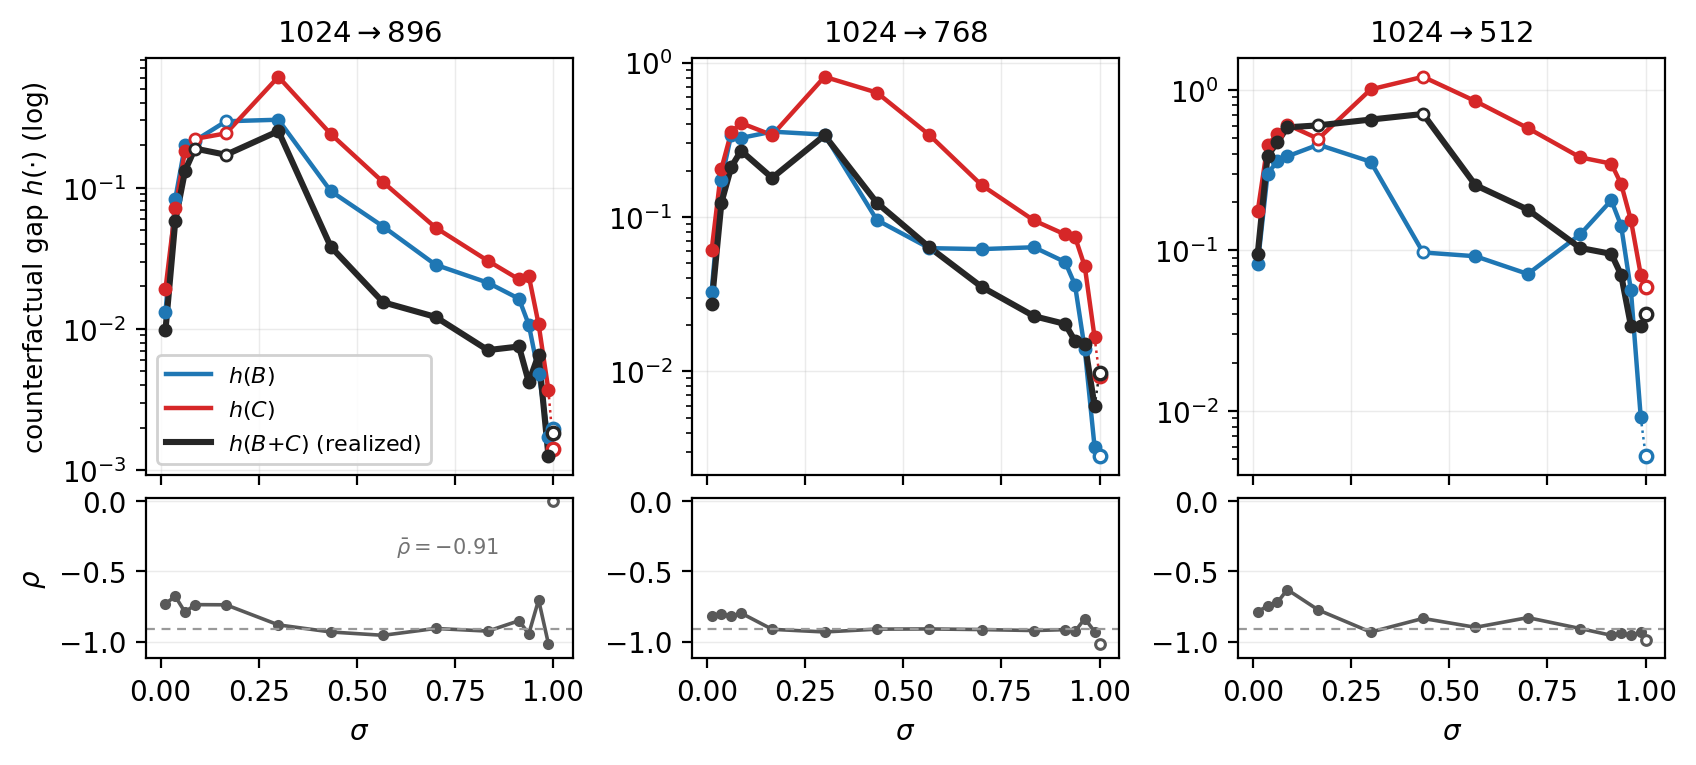
\includegraphics[width=\linewidth]{figs/canc_panel.png}
\caption{\textbf{The gap is the residual of a near-cancellation.}
Per route, the exact counterfactual angles $h(B)$ (data branch
alone), $h(C)$ (graph branch alone), and the realized $h(B{+}C)$
(\;= the measured demotion distance by construction), by $\sigma$
(reenc-referenced vector probe, $N{=}40$, $D{=}12$; gate-failing
bins hollow, $\sigma{=}1$ endpoint detached). The realized curve
sits far below both branches at every measured condition; the lower
strips give the debiased branch anti-alignment
$\rho = \cos(B^{\perp}, C^{\perp})$ per bin, with the pooled
$\bar\rho = -0.91$ dashed.}
\label{fig:canc}
\end{figure}

\begin{figure}[t]
\centering
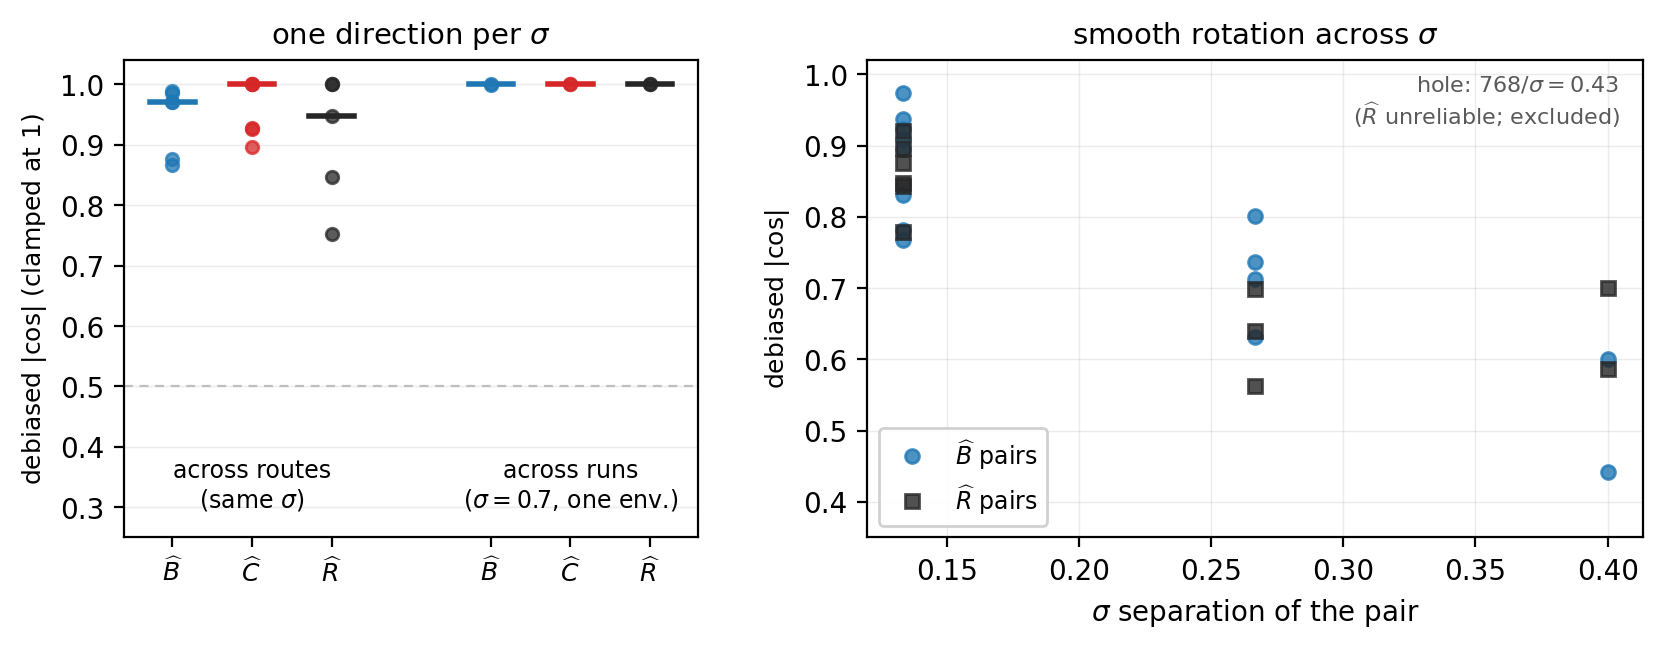
\includegraphics[width=\linewidth]{figs/axis_field.png}
\caption{\textbf{The residual is a $\sigma$-indexed axis field.}
Debiased pairwise cosines between pooled directions across
conditions, by family: across routes at fixed $\sigma$, across two
independent runs at $\sigma = 0.7$ (one shared numerical
environment; \S\ref{sec:instrument}), and across $\sigma$ within one
route, plotted against $\sigma$ separation. One direction per
$\sigma$, shared across routes and runs, rotating smoothly with
$\sigma$; the recorded reliability hole at $768/\sigma = 0.43$ is
marked.}
\label{fig:axisfield}
\end{figure}

\paragraph{The near-cancellation.}
Fig.~\ref{fig:canc} shows $h(B)$, $h(C)$, and the realized
$h(B{+}C)$ per $\sigma$ on each route. At every measured
(route, $\sigma$) both branches are individually far larger than the
realized gap --- on the $896$ route the data branch alone would
realize $104$--$112\%$ of the measured plateau --- and the realized
curve sits far below both: the cancellation removes
${\sim}70$--$77\%$ of the summed branch cost on the safe routes
($1 - h(B{+}C)/(h(B){+}h(C))$ averaged over reliable bins:
$0.77/0.73/0.63$ for $896/768/512$), and at the $768$ window center
the realized gap is ${\sim}25$--$30\%$ of the graph branch's own
angular cost. The anti-alignment behind it is deep everywhere,
$\rho \in [-0.96, -0.63]$, pooling to $\bar\rho = -0.91$ over the
gated verdict bins. The crossing geometry of
\S\ref{sec:ouraccount} reads directly off the amplitude columns: on
$896$, $|B^{\perp}|/|C^{\perp}|$ passes through $1$ within one bin of
the measured mid-$\sigma$ cliff ($\sigma \approx 0.43$--$0.57$); on
$768$ the fine grid shows no in-window crossing --- the ratio rides
at $0.76$--$0.88$ through the window, closest to balance exactly
where the dip sits --- so the $768$ window is the crossing geometry
approached from below rather than crossed. The unsafe route completes
the picture: $512$ keeps the same deep angle
($\mathrm{mean}\,|\rho| \approx 0.86$) while its amplitude ratio
never reaches balance --- what fails on an unsafe route is magnitude
matching, not the cancellation itself.

\paragraph{Where the anti-alignment lives.}
Four targeted reads locate it. \emph{It is born in the pull-back
through $J^{\!\top}$}: the same decomposition applied at the residual
level reads only $\rho_r = -0.12$ to $-0.22$ over the verdict bins,
against $-0.83$ to $-0.96$ in gradient space; a Gaussian spectral
closure derives that weak residual-level seed in sign, shape, and
route ordering (missing its level ${\sim}1.5$--$2\times$), so the
depth of the anti-alignment is a property of the compute graph's
pull-back, not of the data statistics alone. \emph{It is
depth- and type-uniform}: resolved over the network's
$28$~blocks and $15$~module types, every gated cell reads deep
(block-level $\rho_\ell$ median ${\approx}\,{-}0.93$; all module
types $-0.8$ to $-0.97$ where gated, cross-attention and MLP
included), with interaction magnitude proportional to branch energy
at every depth --- no excess interaction anywhere, including the
query/key rows rotary touches directly. \emph{It is locally
enforced}: read per (depth $\times$ module-type) cell, the gated-cell
median $\rho_{\mathrm{cell}}$ is $-0.90$ to $-0.96$ with
interquartile range at most $0.11$ at every verdict $\sigma$ on both
routes --- the pooled constant is not carried by a few cross-cell
modes but holds pointwise in parameter space. \emph{And at
noise-dominated bins it is partially phase-borne}: re-running the
demoted graph with its rotary phases interpolated to match native
geometry rotates the graph branch
($\cos(C^{\perp}, C_{\pi}^{\perp}) = 0.50$--$0.67$ on $768$),
halves the anti-alignment ($\rho \to -0.34$ to $-0.60$), and
\emph{doubles} $h(C)$ --- with phases aligned the graph branch stops
magnitude-matching the data branch, so the phase geometry is part of
what lets the branches cancel. The amplitude of this phase response
concentrates in the adaptive-norm band ($86$--$87\%$), while the
direction rotation is carried globally. Finally, the whole structure
is \emph{operating-point invariant}: re-running the residual-level
probe bit-matched with the adapter merged moves neither branch
(per-image raw $\cos \ge 0.93$ at every gated bin), extending the
checkpoint-controlled replication of Appendix~\ref{app:e7} to the
branch level. Together these reads license quoting $\bar\rho$ as one
constant.

\paragraph{The residual is a $\sigma$-indexed axis field.}
The near-cancellation leaves a residual direction
$\widehat{R} = \widehat{(B{+}C)}$ per (route, $\sigma$), and its legs
$\widehat{B}$, $\widehat{C}$ likewise; comparing them across
conditions (debiased cosines, Fig.~\ref{fig:axisfield}) shows the
residual is not condition-noise. At fixed $\sigma$ the direction is
shared: across routes, median $|\cos| = 0.97$ for the legs and
$0.95$ for $\widehat{R}$ --- $896$ and $768$ demotion push the
adapter along the same line --- and across two independent runs the
debiased cosine is ${\approx}\,1$. The across-run read carries a
scope qualifier: finite-draw directions are compiler-kernel-path
sensitive (\S\ref{sec:instrument}), and the two stores compared
share one numerical environment; cross-environment vector
comparability is not claimed. Across $\sigma$ the axis rotates
smoothly --- adjacent bins $0.89$--$0.97$, decaying monotonically
with $\sigma$ separation to $0.44$--$0.60$ over the widest span,
with no sign flips; a spherical-interpolation check predicts held-out
mid-span directions at median $|\cos| = 0.96$, confirming smoothness
as a description (a parametric rotation law was tested and is
\emph{not} claimed: the best candidate performed worse than
interpolation). Two honest boundaries. First, the rotation is
matched-angle, not planar: the axis rotates through approximately the
same angle as the native gradient direction $\hat g(\sigma)$ itself,
but in its own plane --- transporting a bin's direction by the
anchor's measured rotation buys nothing (median gain $-0.0005$) ---
so the natural reading that the residual simply co-rotates with the
$\sigma$-conditioned native gradient is retired. Second,
reliability: the pooled residual direction passes its
reproducibility gate at $11$ of $12$ verdict conditions; the
exception is $768/\sigma = 0.43$, and mid-window $768$ is generally
where the direction is least reproducible --- the axis-field claims
carry this hole explicitly (supporting panels in
Appendix~\ref{app:geometrypanels}). A decomposition of the residual gap into
its two knobs says which one matters: setting $\rho \to -1$ at
measured amplitudes would remove $70$--$100\%$ of the residual at
every gated condition, while matching amplitudes at the measured
angle removes at most $45\%$ --- the residual gap lives in the
incomplete angle, not in amplitude mismatch.

\paragraph{Closures.}
Four adjacent doors are closed by measurement, and we report them as
results. (1)~\emph{The account's data term is not derivable from the
geometry at the estimand level}: replacing the measured mismatch
curve $x(\sigma)$ with the ledger's own (measured \emph{or}
closure-predicted) branch-amplitude curve fails the held-out lanes at
$4$--$6\times$ the measured lane's RMSE --- and measured and derived
amplitudes fail \emph{equally}, so the failure is an estimand
mismatch between the branch legs and the account's $x(\sigma)$, not
a modeling miss. The same read closes re-deriving any ledger term as
an objective correction. (2)~\emph{Damping-form levers are dead at
probe level}: an exact one-step counterfactual sweep of
adaptive-norm-band damping on the committed stores finds the optimal
damping $\approx$ identity almost everywhere; the entire sweep buys
$\le 0.006$ of gap closure at $13\%$ signal cost. (3)~\emph{A fixed
subspace is refuted at lever level}: projecting out a single shared
residual subspace is actively harmful (signal retention
$0.75$--$0.82$); any projection-style object must be per-$\sigma$-bin.
(4)~Per-sample exploitation of the geometry remains gated on its own
pre-registered chain and is not claimed: every statement above is
about pooled directions at this operating point.

\subsection{Both accounts, scored}
\label{sec:scored}
\label{sec:specscored}
\label{sec:ourscored}

Both accounts are scored against one measured object: the debiased
gap curves of Fig.~\ref{fig:accounts}, read as \S\ref{sec:map} has
just set out. The spectral account is scored first, at the boundary
and then at the curve level; the gradient-perturbation account
follows, term by term.

\paragraph{The spectral account.}
The spectral account's prediction is monotone: the predicted gap is
concentrated at low $\sigma$ and vanishes at high $\sigma$, once
noise drowns the destroyed band (equal-power crossovers
$\sigma \approx 0.14/0.15/0.20$ for $896/768/512$, zero predicted gap
above). The measurement disagrees in both regimes: the transported
curves are near zero precisely where the measured curves peak (RMSE
$0.147$ at $768$, $0.355$ at $512$), and above the crossover the
floor persists (committed-region RMSE $0.027/0.049/0.218$). Neither
read depends on the tolerance or the residual-shape choice in the
transport (within $0.01$ RMSE; Table~\ref{tab:null},
Fig.~\ref{fig:e83}, Appendix~\ref{app:spectral}).


\paragraph{The data branch: a route-uniform residual
mismatch.}
Measuring the mean prediction residual
$\bar r = \mathbb{E}_\epsilon[\hat v - (\epsilon - x)]$ of
\S\ref{sec:reduction} per grid and
$\sigma$ shows a strong,
monotone $\sigma$-shape (cross-grid excess $0.89 \to 0.36$ in
relative $L_2$ from $\sigma{=}0.125$ to $1$) that is the \emph{same
for every route} within $\pm 0.02$, across routes whose gradient
floors span $0$ to $0.3$ (Appendix Table~\ref{tab:residual}). This
result refutes the residual-level prediction of \S\ref{sec:spectral}:
with no cross-frequency coupling, that mismatch is confined to the
destroyed band and ordered by its energy, which differs substantially
across these routes. Route-uniformity implies that the real mismatch
is carried by cross-band structure the diagonal model cannot express,
and that all route identity lives in $J$. The same contrast reads on
assumption~(iv): the measured route-uniformity is the shape
factorization that assumption asserts, established here directly
rather than assumed. The
decay is smooth, Wiener-like shrinkage with no hard gate at the
spectral crossover. How this monotone mismatch, read over the
U-shaped total gradient norm, yields the measured mid-$\sigma$-peaked
curves is a post-hoc consistency read deferred to
Appendix~\ref{app:instrument}.

\paragraph{The graph branch: the floor exists.}
At the $\sigma = 1$ \emph{endpoint} the input-mediated data term is
zero by construction (\S\ref{sec:ouraccount}); the debiased
draw-limit endpoint floors are
$+0.019 / +0.056 / +0.304$ for $896/768/512$ (Appendix
Table~\ref{tab:floor}),
and the $512$ value clears the pre-registered confirmation bar
($\dgap_\infty \ge 0.15$) on $12$ of $12$ probe images individually.
Three companion probes harden this number without adding to it. The
\emph{x-zero} probe reproduces the endpoint floors at every route
(Table~\ref{tab:floor}); a \emph{target-strength sweep} (target
$\epsilon - \alpha x$, $\alpha \in [0, 1]$) finds the paired debiased
excess $\alpha$-flat, discharging the survivor question of
\S\ref{sec:ouraccount} --- the target-mediated gradient is real but
demotion's change to it lands along $\hat g_{\src}$, to which the
angular estimand is blind (Eq.~\ref{eq:exact}); and a forward-only
probe of the model's caption-conditioned \emph{prior} dissociates the
prior from the floors' route ordering, placing the ordering in $J$.
The floor's split into $\mathrm{RoPE}_e + \mathrm{Resid}_e$
(Eq.~\ref{eq:twoterm}) is then read by one origin-side intervention:
evaluating the demoted grid at positionally-interpolated fractional
rotary coordinates, which matches its relative phase geometry to
native, \emph{erases} the $768$ endpoint floor and removes
${\sim}30\%$ of the $512$ floor, the in-band $896$ control untouched
(a raw-estimator probe; \S\ref{sec:limitations}). Re-anchored against
the debiased floors, $\mathrm{Resid}_{768} \approx 0$: what survives
the coordinate fix is the harsh route's
$\mathrm{Resid}_{512} \approx 0.2$ bulk, a genuine non-positional
graph residue, to which the capacity governor below attaches. (The
erasure itself is no training lever; the frequency-selective banded
alignment of \S\ref{sec:trainer} is the form that survives
in-window.) Constructions, anchors, the parallel-landing
decomposition behind the $\alpha$-flatness, and the floor ledger's
full numbers with their per-block depth localization are in
Appendix~\ref{app:instrument}.

\paragraph{The governors: ratio sets the amplitude, absolute size sets
the floor.}
With the floor isolated, what orders the routes? Two probes give a
clean division of labor, and together they decide the equal-ratio
disagreement, limit~(b) of \S\ref{sec:spectral}. \emph{Absolute
size, not ratio, sets the floor}: re-run one tier down, the route
$896{\to}768$ fails its pre-registered bar with a high-$\sigma$
residual ${\sim}2\times$ the $1024{\to}896$ plateau despite a
near-identical downscale ratio, while the two routes sharing the
${\sim}2{,}160$-token target grid, $1024{\to}768$ and $896{\to}768$,
land on the same floor despite different ratios (raw-estimator read,
the separation confirmed by the debiased same-grid floors; Appendix
Table~\ref{tab:phase1a}). Near-equal ratio with a different target
gives a different verdict; the same target with a different ratio
gives the same floor. This refutes any pure ratio rule for the floor,
and with it the spectral account's only degree of freedom. Moreover,
the floor grows monotonically as the \emph{target} grid shrinks
($0.02$--$0.04$ / $0.06$--$0.09$ / ${\approx}\,0.30$ at target
${\sim}3{,}000/2{,}160/1{,}000$ tokens), consistent with the reading
that the floor measures how well the coarse graph approximates the
fine graph's computation.
\emph{Ratio, not absolute size, sets the amplitude}: a synthetic
iso-severity route $1280{\to}1120$, with edge ratio exactly matched to
$1024{\to}896$ at $1.6\times$ its absolute target size, reproduces
the $1024{\to}896$ curve bin-for-bin, crossover included
(raw-estimator read; Appendix Table~\ref{tab:isoseverity}). Note what survives of
the spectral account here: ratio \emph{is} the right governor for the
data term; its error is not its governor but its scope, mistaking one
term for the whole gap.

\paragraph{The cancellation-aware form, at lane parity.}
Since the geometry of \S\ref{sec:observations} suggests an
operational form of its own --- the exact link Eq.~\ref{eq:exact}
evaluated on \emph{both} shares with the interference at the pooled
constant $\bar\rho$ --- we scored it under the identical held-out
protocol as Eq.~\ref{eq:twoterm} (same mismatch curve
bit-identically, same governors, same lanes and bootstrap; only the
link differs). It wins exactly one safe lane: held-out $768$, RMSE
$0.078$ against the additive form's $0.099$, and from held-out
parameters alone it reproduces the measured non-monotone shape and
places the in-window dip at $\sigma = 0.67$ --- the one structure the
additive form cannot express. It loses the other safe lane
(leave-one-out $896$: $0.086$ vs.\ $0.077$) because its graph-side
constant collapses on the $1280$ tier and the cross-tier constant law
does not transfer, and it breaks the guard tier the additive lane
already covers ($1024$ held-out: $0.199$ vs.\ $0.046$). We therefore
report it at lane parity and do \emph{not} adopt it: the additive
lane keeps Fig.~\ref{fig:accounts}, and the reading is that the
interference geometry transfers through governors on the tier that
licensed $\bar\rho$ while its amplitude law across tiers remains
open (demonstration panel and full lane numbers in
Appendix~\ref{app:geometrypanels}).

% Float placed here (end of \S4) purely for pagination: encountered
% on p.9 so it lands atop p.10, next to the \S5 text that reads it.
\begin{table}[t]
\begin{minipage}[t]{0.615\linewidth}
\caption{Weight-space footprint:
$\cos(\Delta W_{\text{arm}}, \Delta W_{\text{native}})$ at matched
training seed, mean $\pm$ SD over three seed pairs, on two
single-artist corpora ($60$/$15$ training images). Training uses
deterministic kernels, including FlashAttention's deterministic
backward \citep{dao2022flashattention} (an identical retrain reads
$1.000$); the
non-det.\ row retrains native at the same seed \emph{without}
deterministic kernels (one twin pair per corpus), so it reads
run-to-run kernel nondeterminism alone. \emph{late}: demotion only in the last
$75\%$ of steps; the stacked row adds the $768$ low-excess window as
a second route ($1024{\to}768$ on $0.65{<}\sigma{<}0.95$, last $50\%$).
\textbf{Bold}: closest endpoints.}
\label{tab:yardstick}
\centering
\footnotesize
\setlength{\tabcolsep}{3pt}
\begin{tabular}{@{}lcc@{}}
\toprule
arm (vs.\ native, matched seed) & corpus A & corpus B \\
\midrule
native, same-seed non-det.\ retrain & $0.264$ & $0.427$ \\
\midrule
$896$, $\sigma{>}0.5$, aligned & $0.365 \pm .020$ & $0.432 \pm .026$ \\
\quad + late & $\mathbf{0.753 \pm .019}$ & $\mathbf{0.770 \pm .009}$ \\
\quad + late, stacked $768$ & $\mathbf{0.753 \pm .017}$ & $\mathbf{0.771 \pm .009}$ \\
$896$, every $\sigma$ & $0.183 \pm .009$ & $0.236 \pm .009$ \\
\bottomrule
\end{tabular}
\end{minipage}\hfill
\begin{minipage}[t]{0.355\linewidth}
\caption{The proposed step, in full. Lines 3--5 (colored) are the
entire change: the gate $\sigmastar{=}0.5$ and the route are read off
the measured map (\S\ref{sec:verdict}), line 5 is the optional
refinement, and lines 1--2 are only a reordering of a standard step,
such that $\sigma$ is drawn before the latent is fetched.}
\label{alg:sigmastep}
\centering
\footnotesize
\setlength{\tabcolsep}{2pt}
\begin{tabular}{@{}>{\ttfamily}r@{~}>{\ttfamily}l@{}}
\toprule
\multicolumn{2}{@{}l@{}}{\textbf{one LoRA training step}} \\
\midrule
1 & $\sigma \sim p_{\mathrm{train}}$ \\
2 & $x \leftarrow$ native latent of $y$ \\
\addedline{3} & \addedline{if $\sigma > \sigmastar$ and $y$ on-route:} \\
\addedline{4} & \addedline{\quad $x \leftarrow$ demoted latent of $y$} \\
\addedline{5} & \addedline{\quad rotary $\leftarrow$ banded$(\sigma)$} \\
6 & $\epsilon \sim \mathcal{N}(0, I)$ at shape$(x)$ \\
7 & $z \leftarrow (1{-}\sigma)x + \sigma\epsilon$ \\
8 & $v \leftarrow \epsilon - x$ \\
9 & step on $\|\hat v_\theta(z, \sigma, c) - v\|^2$ \\
\bottomrule
\end{tabular}
\end{minipage}
\end{table}

